\chapter{Rigid body}

\section{Kinematics}

Let $p_{i}$ represent an arbitrary point on the rigid body 'i' that is 
shown in Figure \ref{fig:rigid_body} and $c_{i}$ the origin of the  
frame $f_{i}$ which is rigidly attached to the body (translates
and rotates with it). The frame $F$ is the inertial frame of reference.

\begin{figure}[h]
    \centering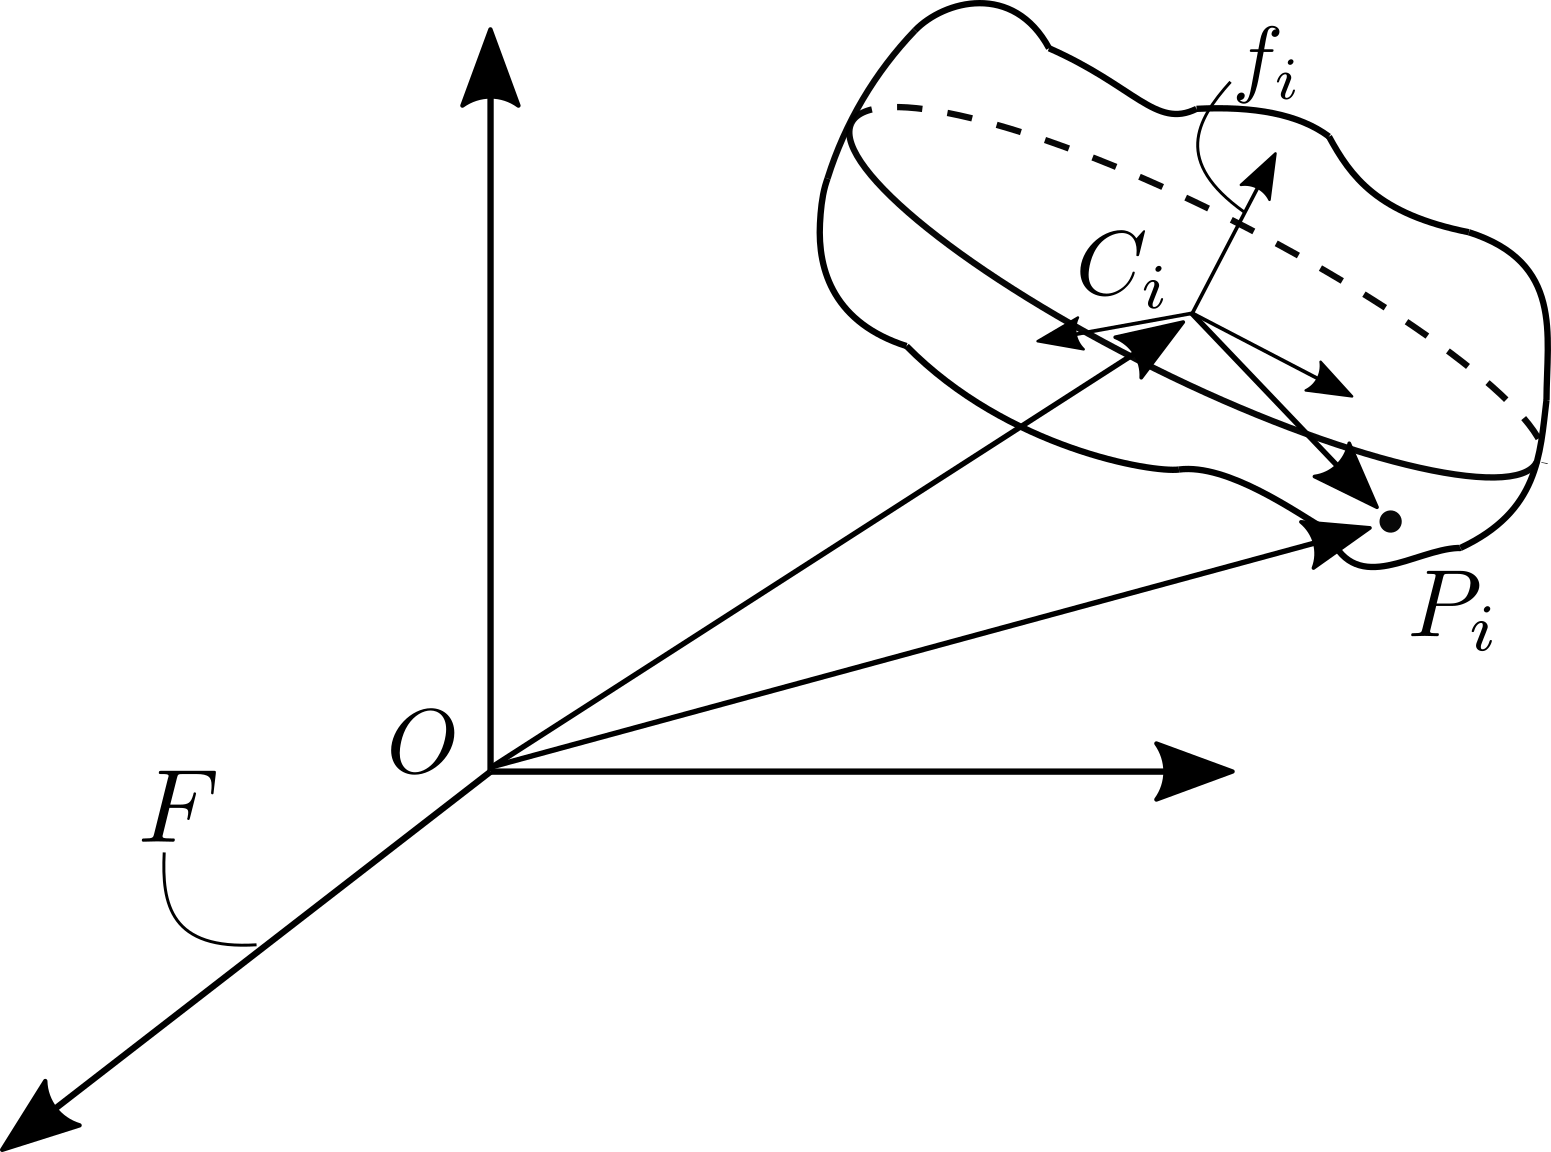
\includegraphics[scale=0.2]{Images/rigid_body_diagram.png}
    \caption{Rigid Body}
    \label{fig:rigid_body}
\end{figure}


\subsection{Position}
The position of the arbitrary point "$p_{i}$" with respect to the inertial frame 
is defined as
\begin{equation}    
    \pvec{r}{op_{i}}{F}{F} = \pvec{r}{oc_{i}}{F}{F} + \rot{R}{f_{i}}{F} \  \pvec{r}{c_{i}p_{i}}{f_i}{f_i},
    \label{eq:position_rigid_body}
\end{equation}

where $\rot{R}{f_{i}}{F}$ is the rotation matrix of body frame $f_{i}$ with respect to 
the inertial frame $F$.

\subsection{Velocity}
The velocity of the the arbitrary point $P_{i}$ with respect to the inertial frame 
is defined as

\[
    \pvec{\dot{r}}{op_{i}}{F}{F} = \pvec{\dot{r}}{oc_{i}}{F}{F} + 
    \frac{d}{dt}(\rot{R}{f_{i}}{F} \  \pvec{r}{c_{i}p_{i}}{f_i}{f_i}),
\]

\begin{equation}
    \pvec{\dot{r}}{op_{i}}{F}{F} = \pvec{\dot{r}}{oc_{i}}{F}{F} + 
    \rot{\dot{R}}{f_{i}}{F} \  \pvec{r}{c_{i}p_{i}}{f_i}{f_i} + 
    \rot{R}{f_{i}}{F} \  \pvec{\dot{r}}{c_{i}p_{i}}{f_i}{f_i}.
    \label{eq:velocity_general}
\end{equation}

We know that for a rigid body the distance between to points remains constant 
meaning that $\pvec{\dot{r}}{c_{i}p_{i}}{f_i}{f_i} = 0$. The time derivative of 
the rotation matrix can be defined as 
\begin{equation}
    \rot{\dot{R}}{f_{i}}{F} = S(\pvec{\omega}{f_{i}}{F}{F}) \ \rot{R}{f_{i}}{F},
    \label{eq:rot_mat_derivative}
\end{equation}

where, $\pvec{\omega}{f_{i}}{F}{F}$ the rotational velocity of $f_{i}$ frame 
with resepct to $F$ frame and $S(\vecd{a})$ skew-symetrix matrix defined as 
\[
    S(\vecd{a}) = \begin{bmatrix}
        0 && -a_{3} && a_{2} \\
        a_{3} && 0 && -a_{1} \\ 
        -a_{2} && a_{1} && 0 \\ 
    \end{bmatrix}, \quad \text{where} \quad \vecd{a} = \begin{bmatrix}
        a_{1} \\ a_{2} \\ a_{3}
    \end{bmatrix}.
\]

Given the above equation \eqref{eq:velocity_general} becomes
\begin{align*}
    \pvec{\dot{r}}{op_{i}}{F}{F} 
    & = \pvec{\dot{r}}{oc_{i}}{F}{F} + 
    S(\pvec{\omega}{f_{i}}{F}{F}) \rot{R}{f_{i}}{F} \ \pvec{r}{c_{i}p_{i}}{f_i}{f_i} \\
    & = \pvec{\dot{r}}{oc_{i}}{F}{F} - S(\rot{R}{f_{i}}{F} \ \pvec{r}{c_{i}p_{i}}{f_i}{f_i}) \ \pvec{\omega}{f_{i}}{F}{F} \\ 
    & = \pvec{\dot{r}}{op_{i}}{F}{F} = \pvec{\dot{r}}{oc_{i}}{F}{F} -
    \rot{R}{f_{i}}{F} \ S( \ \pvec{r}{c_{i}p_{i}}{f_i}{f_i}) \ (\rot{R}{f_{i}}{F})^{T} \ \pvec{\omega}{f_{i}}{F}{F}.  
\end{align*}

or
\begin{equation}
    \pvec{\dot{r}}{op_{i}}{F}{F} = \pvec{\dot{r}}{oc_{i}}{F}{F} - 
    \rot{R}{f_{i}}{F} \ S( \ \pvec{r}{c_{i}p_{i}}{f_i}{f_i})\ \pvec{\omega}{f_{i}}{F}{f_i}.
    \label{eq:velocity_rigid_body}
\end{equation}

It can be proven that the rotational velocity of the body frame with respect to
the inertial frame (expressed in the body frame) can be written as:

\begin{equation}
    \pvec{\omega}{f_{i}}{F}{f_i} = G(\vecd{\theta}_{i}) \ \dot{\vecd{\theta}_{i}} = 
    G_{i} \ \dot{\vecd{\theta}_{i}}, \quad G_{i} = G(\vecd{\theta}_{i}),  
    \label{eq:angular_velocity_expression}
\end{equation}

where $\vecd{\theta}_{i}$ is the vector with the parameters that describe the orientation 
of the body frame with respect to the inertial frame (euler angles, euler parameters,
rodrigues parameters, etc.).

Given expression \eqref{eq:angular_velocity_expression}, equation \eqref{eq:velocity_rigid_body}
becomes    

\[
    \pvec{\dot{r}}{op_{i}}{F}{F} = \pvec{\dot{r}}{oc_{i}}{F}{F} - 
    \rot{R}{f_{i}}{F} \ S( \ \pvec{r}{c_{i}p_{i}}{f_i}{f_i})\ 
    G_{i}\ \dot{\vecd{\theta}_{i}}.
\]

Finally, if we define the generalized rigid body coordinates as 
\begin{equation}
    \vecd{q}_{r_{i}} = \begin{bmatrix}
        \pvec{\dot{r}}{oc_{i}}{F}{F} \\  \vecd{\theta}_{i}
    \end{bmatrix},
    \label{eq:rigid_body_coordinates}
\end{equation}

then equation \eqref{eq:velocity_rigid_body} becomes
\begin{equation}
    \pvec{\dot{r}}{op_{i}}{F}{F} = L_{r}(\vecd{q}_{r_{i}}) \ \dot{\vecd{q}}_{r_{i}},
    \label{eq:velocity_rigid_body_matrix}
\end{equation}

where,
\begin{equation}
    L_{r}(\vecd{q}_{r_{i}}) = L_{r_i} = \begin{bmatrix}
    I_{3 \times 3} && -\rot{R}{f_{i}}{F} \ S( \ \pvec{r}{c_{i}p_{i}}{f_i}{f_i})\ G_{i}         
    \label{eq:lamda_mat_rigid_body}
    \end{bmatrix}.
\end{equation}

\subsection{Acceleration}

The acceleration of the the arbitrary point $P_{i}$ with respect to the inertial frame 
is defined as
    
\begin{align*}
    \pvec{\ddot{r}}{op_{i}}{F}{F} 
    & = \frac{d}{dt}( \pvec{\dot{r}}{oc_{i}}{F}{F} + 
    S(\pvec{\omega}{f_{i}}{F}{F}) \rot{R}{f_{i}}{F} \ \pvec{r}{c_{i}p_{i}}{f_i}{f_i}) \\
    & = \pvec{\ddot{r}}{oc_{i}}{F}{F} +  \pvec{\dot{\omega}}{f_{i}}{F}{F} \times 
    (\rot{R}{f_{i}}{F} \  \pvec{r}{c_{i}p_{i}}{f_i}{f_i}) + 
    \pvec{\omega}{f_{i}}{F}{F} \times 
    \frac{d}{dt}(\rot{R}{f_{i}}{F} \  \pvec{r}{c_{i}p_{i}}{f_i}{f_i}).
\end{align*}

Based on the above, the expression for the acceleration can take the 
following form 
    
\begin{equation}
    \pvec{\ddot{r}}{op_{i}}{F}{F} = \pvec{\ddot{r}}{oc_{i}}{F}{F} +
    \rot{R}{f_{i}}{F} \ S(\pvec{\alpha}{f_{i}}{F}{f_i}) \ \pvec{r}{c_{i}p_{i}}{f_i}{f_i}
    + \rot{R}{f_{i}}{F} \ (S(\pvec{\omega}{f_{i}}{F}{f_i}))^{2} \ \pvec{r}{c_{i}p_{i}}{f_i}{f_i}
    \label{acceleration_rigid_body}
\end{equation}

where 
\begin{equation}
    \pvec{\alpha}{f_{i}}{F}{f_i} = \pvec{\dot{\omega}}{f_{i}}{F}{f_i} = 
    \frac{d}{dt}(G(\vecd{\theta}_{i}) \ \dot{\vecd{\theta}_{i}}) = 
    \dot{G}_{i} \ \dot{\vecd{\theta}_{i}} + 
    G_{i} \ \ddot{\vecd{\theta}_{i}},
    \label{eq:angular_acceleration_expression}
\end{equation}

the expression for the angular acceleration of the body. Substituting 
\eqref{eq:angular_acceleration_expression} into \eqref{acceleration_rigid_body}
leads to 

\begin{align*}
   \pvec{\ddot{r}}{op_{i}}{F}{F} 
   & =  \pvec{\ddot{r}}{oc_{i}}{F}{F} - \rot{R}{f_{i}}{F} \ S(\pvec{r}{c_{i}p_{i}}{f_i}{f_i}) \ \pvec{\alpha}{f_{i}}{F}{f_i}
    + \rot{R}{f_{i}}{F} \ (S(\pvec{\omega}{f_{i}}{F}{f_i}))^{2} \ \pvec{r}{c_{i}p_{i}}{f_i}{f_i} \\ 
    & = \pvec{\ddot{r}}{oc_{i}}{F}{F} - \rot{R}{f_{i}}{F} \ S(\pvec{r}{c_{i}p_{i}}{f_i}{f_i}) (\dot{G}_{i} \ \dot{\vecd{\theta}_{i}} + 
    G_{i} \ \ddot{\vecd{\theta}_{i}}) + \rot{R}{f_{i}}{F} \ (S(\pvec{\omega}{f_{i}}{F}{f_i}))^{2} \ \pvec{r}{c_{i}p_{i}}{f_i}{f_i} 
\end{align*}

or 

\[
    \pvec{\ddot{r}}{op_{i}}{F}{F} = \pvec{\ddot{r}}{oc_{i}}{F}{F} - 
    \rot{R}{f_{i}}{F} \ S(\pvec{r}{c_{i}p_{i}}{f_i}{f_i}) \ \dot{G}_{i} \ \dot{\vecd{\theta}_{i}}
    -     \rot{R}{f_{i}}{F} \ S(\pvec{r}{c_{i}p_{i}}{f_i}{f_i}) \ {G}_{i} \ \ddot{\vecd{\theta}_{i}}
    + \rot{R}{f_{i}}{F} \ (S(\pvec{\omega}{f_{i}}{F}{f_i}))^{2} \ \pvec{r}{c_{i}p_{i}}{f_i}{f_i}  
    \]
If we define 

\begin{equation}    
\vecd{a}_{v_{r_i}}(\vecd{q}_{r_{i}}, \vecd{\dot{q}}_{r_{i}}) = 
    \rot{R}{f_{i}}{F}\ [ (S(\pvec{\omega}{f_{i}}{F}{f_i}))^{2} \ \pvec{r}{c_{i}p_{i}}{f_i}{f_i}  
    - S(\pvec{r}{c_{i}p_{i}}{f_i}{f_i}) \ \dot{G}_{i} \ \dot{\vecd{\theta}_{i}}],
    \label{coriolis_acceleration_rigid_body}
\end{equation}
then the above expression can be written as 

\[    
    \pvec{\ddot{r}}{op_{i}}{F}{F} = \pvec{\ddot{r}}{oc_{i}}{F}{F} 
    - \rot{R}{f_{i}}{F} \ S(\pvec{r}{c_{i}p_{i}}{f_i}{f_i}) \ {G}_{i} \ 
    \ddot{\vecd{\theta}_{i}} + \vecd{a}_{v_{r_i}}(\vecd{q}_{r_{i}}, 
    \vecd{\dot{q}}_{r_{i}}). 
\] 

Using the expression \eqref{eq:lamda_mat_rigid_body} we have 
\begin{equation} 
    \pvec{\ddot{r}}{op_{i}}{F}{F} = L_{r}(\vecd{q}_{r_{i}}) \ 
    \vecd{\ddot{q}}_{r_{i}} + \vecd{a}_{v_{r_i}}(\vecd{q}_{r_{i}}, 
    \vecd{\dot{q}}_{r_{i}}).
    \label{acceleration_rigid_body_matrix}
\end{equation}

\subsection{Virtual Displacement}

We define the virtual displacement of an arbitrary point "$p_{i}$" of the 
rigid body "$i$" as 

\begin{equation}
    \delta \pvec{r}{op_{i}}{F}{F} = \frac{\partial \pvec{r}{op_{i}}{F}{F}}{\partial\vecd{q}_{r_{i}}}
    \ \delta \vecd{q}_{r_{i}}.
    \label{eq:virtual_displacement_in}
\end{equation}

The velocity of this point has previously defined 
(equation \eqref{eq:velocity_rigid_body_matrix}) as 

\begin{align*}
    & \ \pvec{\dot{r}}{op_{i}}{F}{F}  = L_{r}(\vecd{q}_{r_{i}}) \ \dot{\vecd{q}}_{r_{i}} \\ 
    & \Rightarrow  \frac{\partial \pvec{r}{op_{i}}{F}{F}}{\partial t} = 
    L_{r}(\vecd{q}_{r_{i}}) \ \frac{\partial \vecd{q}_{r_{i}}}{\partial t} \\ 
    & \Rightarrow  \frac{\partial \pvec{r}{op_{i}}{F}{F}}{\partial \vecd{q}_{r_{i}}} 
    \frac{\partial \vecd{q}_{r_{i}}}{\partial t} = 
    L_{r}(\vecd{q}_{r_{i}}) \ \frac{\partial \vecd{q}_{r_{i}}}{\partial t}
\end{align*}

For indepedent $\frac{\partial \vecd{q}_{r_{i}}}{\partial t}$ it is obvious that 

\begin{equation}
    \frac{\partial \pvec{r}{op_{i}}{F}{F}}{\partial \vecd{q}_{r_{i}}}
    = L_{r}(\vecd{q}_{r_{i}}).
    \label{eq:virtual_displacement_partial}
\end{equation}

Combining equations \eqref{eq:virtual_displacement_in} and 
\eqref{eq:virtual_displacement_partial} we define the virtual displacement of 
point $p_{i}$ as  

\begin{equation}
    \delta \pvec{r}{op_{i}}{F}{F} = L_{r}(\vecd{q}_{r_{i}})\ \delta \vecd{q}_{r_{i}}
    \label{eq:virtual_displacement}
\end{equation}

%%%%%%%%%%%%%%%%%%%%%%%%%% Dynamics %%%%%%%%%%%%%%%%%%%%%%%%%%%%%%%%%%5
\section{Dynamics}

There are several methods for developing the dynamic equations of motion of
the rigid bodies. In this section, the \textit{principle of virtual work in dynamics} 
will
be used to obtain the differential equations that govern the spatial motion of
the rigid bodies. Based on D'Alembert's principle, a body "$i$" (rigid or flexible) 
in a dynamic equilibrium obeys the following equation

\begin{equation}
    \delta W^{e}_{i} = \delta W^{in}_{i},
    \label{eq:principle_of_virtual_work}
\end{equation}

where, $\delta W^{e}_{i}$ is the virtual work of the externaly applied forces 
to the body and $\delta W^{in}_{i}$ is the virtual work the the inertial forces.

\subsection{Virtual work of inertial forces}
For a continuum the virtual work of inertial forces is defined as 

\begin{equation}
    \delta W^{in}_{i} = 
    \int_{m_i} \pvec{\ddot{r}}{op_{i}}{F}{F} \  \delta\pvec{r}{op_{i}}{F}{F} \ dm_{i},
    \label{eq:virtual_work_inertial_definition}
\end{equation}

where $p_i$ is an arbitrary point of the body $"i"$.

For a rigid body it has proven that 

\[
    \pvec{\ddot{r}}{op_{i}}{F}{F} = L_{r}(\vecd{q}_{r_{i}}) \ 
    \vecd{\ddot{q}}_{r_{i}} + \vecd{a}_{v_{r_i}}(\vecd{q}_{r_{i}}, 
    \vecd{\dot{q}}_{r_{i}}) \quad \text{and} \quad \delta \pvec{r}{op_{i}}{F}{F} 
    = L_{r}(\vecd{q}_{r_{i}})\ \delta\vecd{q}_{r_{i}}
\]

Combining the above with equation \eqref{eq:virtual_work_inertial_definition} 
the virtual work of inertial forces can be written as 

\[
    \delta W^{in}_{i} = 
    \vecd{\ddot{q}}_{r_{i}}^{T}\ \int_{m_i} (L_{r_i})^{T} \ L_{r_i}\ dm_{i}\ \delta\vecd{q}_{r_{i}} 
    + \int_{m_i} \vecd{a}_{v_{r_i}}\ L_{r_i}\ dm_{i}\ \delta\vecd{q}_{r_{i}} 
\]

If we define the mass matrix ,
\begin{equation}
    M_{r_i} = \int_{m_i} (L_{r_i})^{T} \ L_{r_i}\ dm_{i},
    \label{eq:mass_matrix_rigid_body}
\end{equation}
and the centrifugal-coriolis forces vector
\begin{equation}
    \vecd{f}_{v_{r_i}} = \vecd{f}_{v_{r_i}}(\vecd{q}_{r_{i}}, 
    \vecd{\dot{q}}_{r_{i}}) = - \int_{m_i} (L_{r_i})^{T} \ \vecd{a}_{v_{r_i}}\ 
    \ dm_{i},
    \label{eq:coriolis_forces_rigid_body}
\end{equation}

then the equation above becomes

\begin{equation}
    \delta W^{in}_{i} = (\vecd{\ddot{q}}_{r_{i}}^{T}\ M_{r_i}  
    - \vecd{f}_{v_{r_i}}^{T})\delta\vecd{q}_{r_{i}}.
    \label{eq:virtual_inertial_work_rigid_body}
 \end{equation}



\subsubsection{Mass matrix}
In equation \eqref{eq:mass_matrix_rigid_body}, the mass matrix of the rigid 
body was defined as 
\[
    M_{r_i} = \int_{m_i} (L_{r_i})^{T} \ L_{r_i}\ dm_{i}.
\]   

Given equation \eqref{eq:lamda_mat_rigid_body}, this expression can be 
formulated as 

\begin{align*}
M_{r_i} & = \int_{m_i} \begin{bmatrix}
    I_{3 \times 3} \\ -G^{T}_{i}\ (S(\pvec{r}{c_{i}p_{i}}{f_i}{f_i}))^{T}\ \rot{R}{F}{f_i}         
    \end{bmatrix}\ \begin{bmatrix}
    I_{3 \times 3} && -\rot{R}{f_{i}}{F} \ S( \ \pvec{r}{c_{i}p_{i}}{f_i}{f_i})\ G_{i}         
    \end{bmatrix}\ dm_{i} \\ 
    & = \int_{m_i} 
    \begin{bmatrix}
    I_{3 \times 3} && -\rot{R}{f_{i}}{F}\ S(\pvec{r}{c_{i}p_{i}}{f_i}{f_i})\ G_{i}
    \\ -G^{T}_{i}\ (S(\pvec{r}{c_{i}p_{i}}{f_i}{f_i}))^{T}\ \rot{R}{F}{f_i} && 
    G^{T}_{i}\ (S(\pvec{r}{c_{i}p_{i}}{f_i}{f_i}))^{T}\ S(\pvec{r}{c_{i}p_{i}}{f_i}{f_i})\ G_{i}        
    \end{bmatrix}\ dm_{i} \\ 
    & = \begin{bmatrix}
        m^{r_i}_{11} && m^{r_i}_{12} \\ m^{r_i}_{21} && m^{r_i}_{22}
    \end{bmatrix}
\end{align*}

where,

\begin{subequations}
\begin{align}
    m^{r_i}_{11} &= \int_{m_i} I_{3 \times 3}\ dm_{i} =  m_{i} I_{3 \times 3} \\
    m^{r_i}_{12} &= (m^{r_i}_{21})^{T} = -\rot{R}{f_{i}}{F}\ \int_{m_i} S(\pvec{r}{c_{i}p_{i}}{f_i}{f_i})\ dm_{i}\ G_{i}\\ 
    m^{r_i}_{22} &= G^{T}_{i}\ \int_{m_i} (S(\pvec{r}{c_{i}p_{i}}{f_i}{f_i}))^{T}\ S(\pvec{r}{c_{i}p_{i}}{f_i}{f_i})\ dm_{i}\ G_{i}
\end{align}
    \label{eq:mass_matrix_components_rigid_body}
\end{subequations}

We define the body's inertial tensor on the point $c_i$ and with respect to 
the body frame $f_i$ as 

\begin{equation}
    I_{c_i}^{f_i} = \int_{m_i} (S(\pvec{r}{c_{i}p_{i}}{f_i}{f_i}))^{T}\ S(\pvec{r}{c_{i}p_{i}}{f_i}{f_i})\ dm_i .
    \label{eq:inertial_tensor_rigid_body}
\end{equation}

Given that the frame $f_i$ is rigidly attached to the body the above inertial 
tensor remains constant for the rigid body case. Then we have 
\begin{equation}
    M_{r_i} = \begin{bmatrix}
        m_{i}\ I_{3 \times 3} && m_{12} \\ m_{21} && G^{T}_{i} \ I^{f_i}_{c_i}\ G_i
    \end{bmatrix}.
    \label{eq:mass_matrix_rigid_body}
\end{equation}



\subsubsection{Centrifugal-coriolis forces vector}
The vector of centrifugal-coriolis forces was given by the equation 
\eqref{eq:coriolis_forces_rigid_body} as
\[
    \vecd{f}_{v_{r_i}}(\vecd{q}_{r_{i}}, 
    \vecd{\dot{q}}_{r_{i}}) = - \int_{m_i} (L_{r_i})^{T} \ \vecd{a}_{v_{r_i}}\ 
    \ dm_{i}
\]
% Furthermore, in the case that $c_{i}$ is the center of mass of the body $"i"$ then it
%  can be defined as
% \[
%     \pvec{r}{oc_{i}}{F}{F} = \frac{1}{m_{i}}\int_{m_i} \pvec{r}{op_{i}}{F}{F} \  dm_{i}
%     \quad \text{where} \quad m_{i} = \int_{m_i} dm_{i}.
% \]
% Given the above equations it is easily proven that 
% \begin{align*}
%     \int_{m_i} \pvec{r}{c_{i}p_{i}}{f_i}{f_i}\ dm_{i} 
%     & = \rot{R}{F}{f_i}\int_{m_i} \pvec{r}{c_{i}p_{i}}{f_i}{F}\ dm_{i} \\ 
%     & = \rot{R}{F}{f_i}(\int_{m_i} \pvec{r}{o_{i}p_{i}}{F}{F}\ dm_{i} - 
%     \int_{m_i} \pvec{r}{o_{i}c_{i}}{F}{F}\ dm_{i}) \\
%     & = \rot{R}{F}{f_i}(m_{i}\ \pvec{r}{o_{i}c_{i}}{F}{F} - 
%     \pvec{r}{o_{i}c_{i}}{F}{F} \int_{m_i} \ dm_{i}) \\
%     & = \vecd{0}.
% \end{align*}

% From the equations above it is obvious that in the case that $c_i$ is the center 
% of mass of the rigid body
% \begin{equation}
%     m^{r_i}_{12} = (m^{r_i}_{21})^{T} = 0. 
%     \label{eq:mass_matrix_rigid_centrifugal_body}
% \end{equation}

% From equations \eqref{eq:mass_matrix_components_rigid_body}, 
% \eqref{eq:inertial_tensor_rigid_body} and 
% \eqref{eq:mass_matrix_rigid_centrifugal_body} we can define the mass matrix of 
% a rigid body as 

% \begin{equation}
%     M_{r_i} = \begin{bmatrix}
%         m_{i}\ I_{3 \times 3} && 0 \\ 0 && G^{T}_{i} \ I^{f_i}_{c_i}\ G_i
%     \end{bmatrix},
%     \label{eq:mass_matrix_rigid_body}
% \end{equation}
% where $c_i$ is the center of mass of body $"i"$.

